\documentclass[11pt]{scrartcl}
\usepackage[ngerman]{babel}
\usepackage[utf8]{inputenc}
\usepackage[a4paper,lmargin={2.5cm},rmargin={2.5cm},tmargin={2.5cm},bmargin={2.5cm}]{geometry}
\usepackage{graphicx}
\usepackage[T1]{fontenc}
\usepackage[headsepline,footsepline, singlespacing=true]{scrlayer-scrpage}
\usepackage{mwe}
\usepackage{acro}
\usepackage{blindtext}
\usepackage[hidelinks]{hyperref}
\usepackage{csquotes}
\usepackage{setspace}
\usepackage[ngerman]{cleveref}
\usepackage[ngerman]{todonotes}
\usepackage{graphicx}
\usepackage{lmodern}
\usepackage{tocloft}
\usepackage{microtype}
\usepackage{longtable}
\usepackage{tabu}
%\usepackage{supertabular}

\usepackage[
  backend=biber,
  style=ext-authoryear,
  maxcitenames=2, maxbibnames=999,
  giveninits=true,
  url=false,
  uniquename=init, uniquelist=false,
  articlein=false, innamebeforetitle=true,
  punctfont=true, dashed=false,
]{biblatex}

%\setkomafont{disposition}{\normalcolor\bfseries} %Überschriften afu standardschrift stellen, hässlich bei einer Schrift mit Serifen
\setkomafont{caption}{\bfseries} %captio Abbilund und Tabbellen beschriftung!
\setkomafont{captionlabel}{\bfseries}
\setcaptionalignment{l}

\DefineBibliographyStrings{ngerman}{
	andothers = {{et\,al\adddot}}
}

\renewcommand{\cftfigpresnum}{Abbildung\space}
\renewcommand{\cftfignumwidth}{2.5cm}
\renewcommand{\cftfigaftersnum}{:}
\newcommand{\fontForTheSeminar}{ppl}
\newcommand{\fontForHeadlines}{lmss}
\renewcommand*{\mkbibnamefamily}{\expandafter\MakeUppercase\expandafter}
\AtBeginBibliography{%
  \renewcommand*{\mkbibnamefamily}[1]{#1}}

\DeclareNameFormat{labelname}{%
  \ifnum\value{uniquename}=0\relax
    \usebibmacro{name:family}
      {\namepartfamily}
      {\namepartgiven}
      {\namepartprefix}
      {\namepartsuffix}%
  \else
    \usebibmacro{name:family-given}
      {\namepartfamily}
      {\namepartgiveni}
      {\namepartprefix}
      {\namepartsuffixi}%
  \fi
  \usebibmacro{name:andothers}}

\DeclareNameAlias{default}{family-given}
\DeclareNameAlias{sortname}{default}

\DeclareDelimAlias*[bib]{finalnamedelim}{multinamedelim}
\setlength{\bibhang}{0pt}

\DeclareNameWrapperFormat{sortname}{\mkbibbold{#1}}
\DeclareFieldFormat{biblabeldate}{\mkbibbold{\mkbibparens{#1}}}
\DeclareFieldFormat{journaltitle}{#1\isdot}
\DeclareFieldFormat*{title}{#1}

\DeclareDelimFormat[bib]{nametitledelim}{\addcolon\space}

\renewcommand*{\volnumdelim}{\addcomma\space}
%\renewcommand*{\issnumdelim}{\addcolo\space}

%\renewcommand*{\yearpagesdelim}{\addcolon\space}

\DeclareFieldFormat{pages}{#1}

\renewcommand*{\bibpagespunct}{\addcolon\ifentrytype{article}{\space}{\space}}

\DeclareDelimFormat{postnotedelim}{\addcolon~}
\DeclareFieldFormat{postnote}{\mknormrange{#1}}
\setlength\bibitemsep{6pt}

\renewcommand*{\bibfont}{\normalsize}

%Schriftwahl
\newcommand{\changefont}[3]{\fontfamily{#1} \fontseries{#2} \fontshape{#3} \selectfont}


\addbibresource{bibtex/bib.bib}

\setlength{\parindent}{0pt}
\RedeclareSectionCommand[%
	beforeskip=32pt,
	afterskip=6pt,
	runin=false]{section}

\RedeclareSectionCommand[%
	beforeskip=12pt,
	afterskip=6pt,
	runin=false]{subsection}

\RedeclareSectionCommand[%
	beforeskip=12pt,
	afterskip=6pt,
	runin=false]{subsubsection}

\pagestyle{scrheadings}
\changefont{\fontForTheSeminar}{m}{n}
\linespread{1.3}
\flushbottom
%Abkürzungen definieren!

\DeclareAcronym{NEA}{
	short = NEA,
	long = Netzersatzanlage
}

\DeclareAcronym{CSR}{
	short = CSR,
	long = Corporate Social Responsibility
}

\DeclareAcronym{KWK}{
	short = KWK,
	long = Kraftwärmekopplung
}

\DeclareAcronym{EEG}{
	short = EEG,
	long = Erneuerbare-Energien-Gesetz
}

\acsetup{
  make-links ,
%  list / template = tabular 
  index ,
%  pdfcomments/use = true ,
  trailing/activate = {dash} 
}
\title{PV Gruppe 1}
\author{Annika Kruse, Sophie Feye, Tibor Weiß, Tu Ly}
\begin{document}
\maketitle
\newpage
%\changefont{\fontForHeadlines}{m}{n}
%\setkomafont{section}{15}
%\setkomafont{subsection}{14}
%\setkomafont{subsubsection}{13}


%einige letzte Befehle für das Layout
\newpage %neue Seite nach dem DEckblatt
\clearpairofpagestyles %alle Layouteinstellungen vom Deckblatt löschen
\ohead{\headmark} %Kopfzeile
\ofoot{\pagemark} %Fußzeile
\automark{section} %aktuelle Section wird in der Kopfzeile angezeigt
\renewcommand*{\sectionmarkformat}{}%\changefont{\fontForHeadlines}{m}{n}} %Darstellung Section in der Kopfzeile angepasst
%\renewcommand{\sectionmarkformat}{\changefont{\fontForHeadlines}{m}{n}}
\setcounter{page}{2} %Seitenzähler auf 2 Stellen
\setlength{\parskip}{9pt} %Abstand nach Absatz
\changefont{\fontForTheSeminar}{m}{n} %Schrift aktualisieren
%\renewcommand{\figurename}{Abbildung}
%Inhaltsverzeichnis
\tableofcontents
%\addcontentsline{toc}{section}{Inhaltsverzeichnis}


\newpage
%Tabellen- und Abbildungsverzeichnis
\addcontentsline{toc}{section}{Tabellenverzeichnis}
\listoftables
\addcontentsline{toc}{section}{Abbildungsverzeichnis}
\listoffigures
%Anhangsverzeichnis 
%\todo{Tabellen und Anhangsverzeichnis erstellen! Formatierung vorgaben einsehen!}

%Abkürzungsverzeichnis - Abkürzungen eintragen
%\section*{Abkürzungsverzeichnis}

\addcontentsline{toc}{section}{Abkürzungsverzeichnis}
\printacronyms[
 heading = section* ,
 name = Abkürzungsverzeichnis ,
 display = used,
% sort 
% template = tabular ,
 template = longtabu
]
\newpage

\section{Einleitung}
\todo{Annika}

\section{Poltische Situation und gesetzliche Lage}
\todo{Zitate über cite einbinden!}
Um dem Klimawandel entgegen zu wirken, wurde im Juni 2021 ein neues Bundes-Klimaschutzgesetz vom Deutschen Bundestag beschlossen.
Es verschärft die bislang geltenden Ziele und strebt eine Treibhausgasneutralität bis 2045 an.
Die Reduktion ist nach einzelnen Sektoren aufgeteilt (siehe \cref{fig:CO2}).
Als Hilfe zur Umsetzung des geplanten Maßnahmen wurde ebenfalls ein Klimaschutzsofortprogramm 2022 von der Bundesregierung verabschiedet.
Dieses bietet die Bereitstellung von zusätzlichen 8 Mrd. € an, um alle Sektoren, aber vor allem die Industrie, die Gebäude und die Energiewirtschaft zu unterstützen.
\cref{fig:CO2} veranschaulicht die angestrebte Reduzierung der Treibhausgase um etwa 56,5 \% von 1990 bis 2030.
Dieses Ziel soll allein mit einer Senkung der Emissionen aus der Energiewirtschaft zur Hälfte erfüllt werden (BMWi 2021).
Bis 2016 wurde in diesem Sektor allerdings erst 42 \% der angestrebten Minderung erreicht (BMUV 2020).

Trotzdessen wurden gesetzlich festgelegten Ziele für den Ausbau von Photovoltaik 2021 in Deutschland eingehalten.
Es ist zu erwarten, dass die Klimaneutralität im Sektor Energiewirtschaft früher erreicht wird als angenommen.
Hierfür ist jedoch ein massiver Ausbau erforderlich (WIRTH 2021: 6).


\begin{figure}
\centering
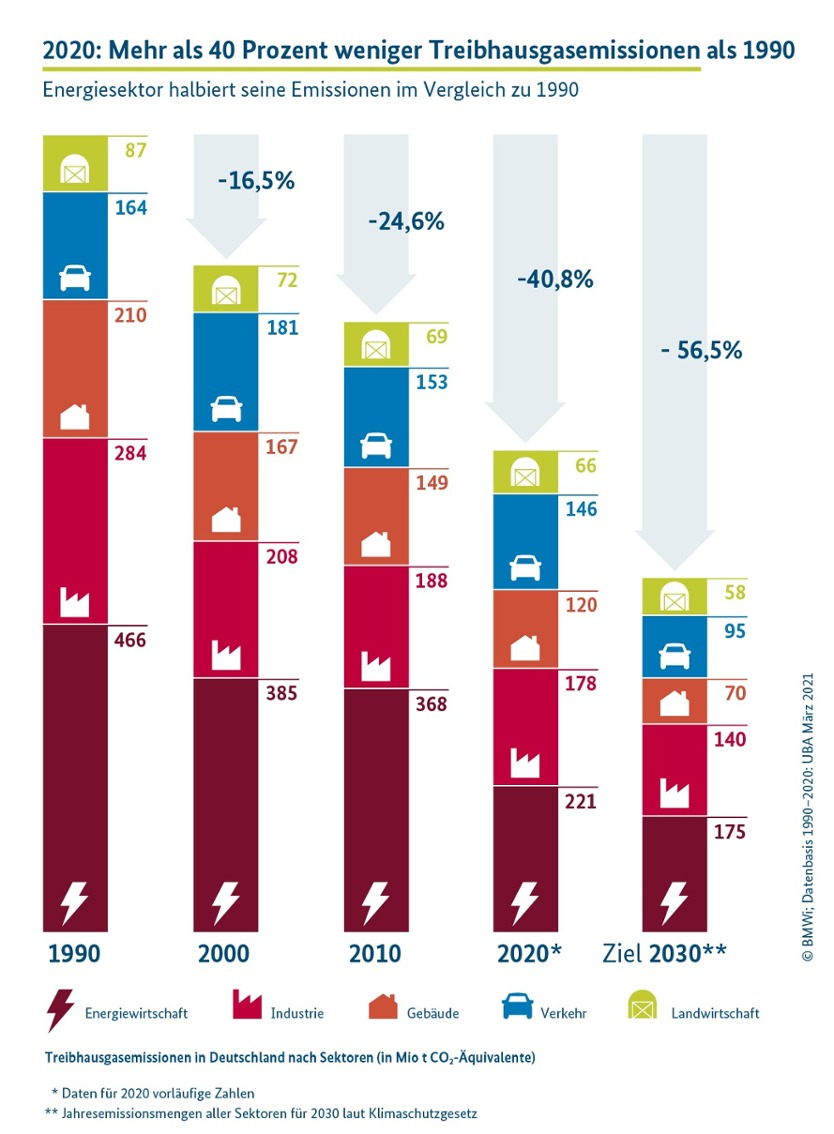
\includegraphics[width=0.8\textwidth]{Sophie/co2.jpg}
\caption[Treibhausgasemissionen in Deutschand nach Sektoren in Mio. t CO\textsubscript{2}-Äquivalente von 1990 bis 2030]{Treibhausgasemissionen in Deutschand nach Sektoren in Mio. t CO\textsubscript{2}-Äquivalente von 1990 bis 2030 (BMWi 2021)}
\label{fig:CO2}
\end{figure}

Um die Klimaziele zu erfüllen, sind allerdings weitere Maßnahmen zur Förderung von Erneuerbaren Energien notwendig.
Die Photovoltaik-Leistung in Deutschland setzt sich zu 3/4 aus Dachanlagen und 1/4 aus Freiflächenanlagen zusammen.
Die kontinuierliche Leistungssteigerung der Freiflächenanlagen bietet die Möglichkeit, dass immer weniger Fläche für höhere Erzeugnisse an Solarstrom benötigt wird.
Bis 2020 standen für die Anlagen 30.000 ha Fläche in Deutschland zur Verfügung.
0,07 \% der landwirtschaftlich genutzten Fläche wurde unter anderem für den Aufbau umgenutzt (UMWELT BUNDESAMT 2021).

Zur Förderung der Energiewende und der Investionen in PV-Anlagen gibt es das \ac{EEG}.
Ziel ist es, die Stromgestehungskosten aus Erneuerbaren Energien kontinuierlich zu reduzieren.
Das \ac{EEG} ermöglicht den Anlagenbetriebern einen angemessenen Gewinn bei einer garantierten Stromabnahme.
Die Stromgestehungskosten setzen sich dabei aus dem Verhältnis der elektrischen Energieproduktion und den Gesamtkosten zusammen.
Gesamtkosten umfassen bei PV-Anlagen die Anschaffungskosten, Finanzierungsbedingungen, Betriebskosten während des Nutzungszeitraumes und die Rückbaukosten (WIRTH 2021: 8 f.).

Nach dem \ac{EEG} (2021 §6) kann der betroffenen Gemeinde eine finanzielle Beteiligung an den Erlösen von Freiflächenanlagen in Höhe von von 0,2 ct/ kWh vom Anlagenbetreiber angeboten werden.
Da der Bau genehmigungspflichtig ist, können zusätzliche Auflagen hinsichtlich Höhe der Gestelle oder Ausgleichsflöchen von der Gemeinde erfolgen.
Nach §19 des \ac{EEG} 2021 haben die Anlagenbetreiber gegenüber dem Netzbetreiber einen Anpruch auf eine Marktprämie, eine Einspeisevergütung oder einen Mieterstromzuschlag.
Des Weiteren gibt es Vorgaben zur Errichtung von PV-Freiflächenanlagen.
Die Anlagen dürfen nur auf Ackerland entlang von Autobahnen oder Schienen in 200-m-Korridoren erreichtet werden sowie auf Konversions- und bereits versiegelten Flächen.
Außerdem ist die Größe auf 20 MW begrenzt (EEg 2021: §37).
Bei einem Eigenverbrauch aus PV-Anlagen ab etwa 30 kW Nennleistung muss eine Abgabe von 40 \% der aktuellen \ac{EEG}-Umlage erfolgen.
Anlagen mit Nennleistungen von 750 kW bis 20 MW dürfen nicht mehr zur Eigenversorgung genutzt werden (WIRTH 2021: 10).

Entscheidend für die Förderung der PV-Anlagen ist die oben genannte Einspeisevergütung.
Sie fördert Anlagen in einem Zeitraum vom 20 Jahren, zuzüglich der Monate bis zum Jahresende nach dem Bau.
Die Förderung kann allerdings nur von Betreibern in Anspruch genommen werden, die den gesamten erzeugten Strom an den Netzbetrieber übergeben und weniger als 10 MWp leisten (EEG 2021: §20).



\section{Methoden und betriebswirtschaftliche Annahmen}
\todo{Stromverbrauch Tibor}
\todo{treurat+Partner Sophie Stromertrag}
\todo{Methoden Sophie}

\section{Betriebliche Situation}
\label{sec:betrieb}
\todo{Tibor}

Der landwirtschaftliche Betrieb \textit{Heuwirtschaft Wildenhorst} hat sich auf die Produktion und dem Verkauf von hochwertigem Heu spezialisiert.
Dafür wird eine Heutrocknung betrieben, welche einen gewissen Energiebedarf hat.
Derzeit benötigen 2 Lüfter jeweils 37 kW\textsubscript{el} und der Entfeuchter 90 kW\textsubscript{el} sowie eine Anwärmung der Luft mit ca. 100 bis 300 kW\textsubscript{Wärme} über Solarthermie (Absaugung der Luft zwischen Blechdach und OSB Innenverkleidung) und Abwärme der \ac{NEA}.

\subsection{Saisonaler Energiebedarf}
Die Trocknung des Heus hängt natürlich von der Vegetationszeit des Grases ab, sodass die Trocknung von Mitte Mai bis Anfang September nahezu komplett ausgelastet ist und in den nächsten vier bis fünf Wochen nur zweimal für etwa 100 Stunden eingeschaltet wird.
Die Trocknung muss Tag und Nacht laufen, da durch den trockenen Luftstrom die Qualität des Heus gesichert wird.
Eine Verlängerung der Trocknugnszeit ist keine Option, da bei einer zu langen Trocknungszeit die Qualität leidet und der Durchsatz der Trocknungsanlage reduziert wird.

\subsection{Derzeitige Energieversorgung}
Auf den großen Dachflächen der neueren Gebäude (BJ ab 2012, ca. 3000 m\textsuperscript{2}) wurde, aufgrund der geringen Einspeisevergütung und der teilweisen Nutzung der Solarthermie, bisher keine Photovoltaikanlage installiert.
Des weiteren kann ein Eigenverbrauch von Solarstrom nicht, bzw. nur mit hohem Aufwand (siehe \cref{subsec:NEA}), umgesetzt werden, da über eine vorhandene \ac{NEA} günstig Strom erzeugt werden kann \footnote{Aus 1 l Heizöl können 4 kWh Strom gewonnen werden}.
Die Abwärme der \ac{NEA} wird dem Trocknungskreislauf zugeführt und steigert somit den Wirkungsgrad erheblich.

Eine Nutzung des Stromnetzes für die Trocknung ist derzeit für den Betrieb sehr teuer.
Die Entscheidung zur Nutzung einer \ac{NEA} wurde 2017 getroffen, zu diesem Zeitpunkt war, aufgrund der hohen Spitzenlast, die jährliche Grundgebühr bei etwa 10.000 € und der Arbeitspreis mit allen Abgaben bei knapp 30 ct/kWh.\todo{überprüfen!}
Der Arbeitspreis ist so hoch aufgrund der hohen Volatilität der Stromabnahme, welche es für den Energieversorger schwer macht, die Stromabnahme einzuschätzen.
Daher ist eine Energieeigenversorgung im Bereich der Trocknung anzustreben.

In der Kombination mit der \ac{KWK} ist die Verwendung einer \ac{NEA} daher für den Betrieb aktuell eine sehr günstige Variante der Energieversorgung.
Zu Beachten ist auch die Stundenzahl von knapp 2.000 Betriebsstunden im Jahr, welche für eien gute Verteilung der Fixkosten sorgt, aber gering genug ist um eine lange Lebensdauer zu ermöglichen.
Mit Einflussfaktoren wie den  Klimawandels und \ac{CSR} ist die Verbrennung von Heizöl zur Stromerzeugung keine zukunftsfähige Lösung.

\subsection{Besonderheiten NEA}
\label{subsec:NEA}
Eine \ac{NEA} kann, wie in diesem Fall, in einem Inselbetrieb laufen.
In so einem Fall, hat die \ac{NEA} keine Verbindung mit dem Stromnetz und braucht, wenn nur ein Generator vorhanden ist, keine Aufwändige Synchronisierung mit anderen Erzeugern.
Eine Aufrüstung für die Möglichkeit der Synchronisierung würde im Bereich der \ac{NEA} eine Investition von etwa 10.000 € bedeuten.
Wenn die \ac{NEA} mit dem Stromnetz verbunden sein soll, müssen dafür Genehmigungen bei dem Netzbetreiber eingeholt werden und viele Auflagen beachtet werden.


\subsection{Flächeneignung für Photovoltaik}
Neben der Trocknugnshalle steht eine betriebseigene Fläche mit etwa 3 ha landwirtschaftlicher Nutzfläche zur Verfügung.
An dieser Fläche führt ein Feldweg vorbei, sonstige Anlieger sind ein landwirtschaftlicher Betrieb, ein Altenteilhaus sowie weitere landwirtschaftliche Nutzflächen.
Hierbei handelt es sich nicht um Wohngebiete sondern um Außenbereiche mit den entsprechenden Richtlinen.
Die Gemeinde profitiert bei dem Bauvorhaben nicht nur durch entsprechende Einnahmen, sondern auch, dass im Sommer die Geräusche der \ac{NEA} wegfallen würde.



\section{Gesamtkonzept}
\todo{Tibor}
Die günstige Energieversorgung für den Betrieb wird unter dem Gesichtspunkt der steigenden Energiepreise eine zentrale Herausforderung für den wirtschaftlichen Erfolg sein.
Auch wenn derzeit eine Nutzung von fossilen Energieträgern die günstigste Variante ist, wird dies, aufgrund der Politik, welche die CO\textsubscript{2}-Emissionen in den nächsten zehn Jahren deutlich reduzierne will, nicht zwangläufig bleiben.\todo{cite!}
Aufgrund der besonderen Anforderungen, siehe \cref{sec:betrieb}, wäre eine Kombination von Photovoltaik und Stromspreicher eine mögliche Alternative.
Mit den stark fallenden Preisen für Stromspeicher \todo{cite!} und steigenden Kraftstoffpreisen wird es einen Zeitpunkt geben, bei welchem die beschriebene Investition wirtschaftliche Vorteile bringt.

\subsection{Marketing}
Die \textit{Heuwirtschaft Wildenhorst} vermarktet, wie in \cref{sec:betrieb} beschrieben, hochwertiges Heu.
Bei hochwertigen Produkten spielt neben der Qualität auch das Image des Herstellers eine wichtige Rolle.
In diesem Zusammenhang sind \ac{CSR} Maßnahmen als sinnvoll zu erachten.
So wurde im Herbst 2019 der Verein \textit{Wildtierrettung Wildenhorst e.V.} gegründet, welcher von der \textit{Heuwirtschaft Wildenhorst} eine großzügige Spende erhalten hat.
So konnte bereits im Frühjahr 2020 mit Hilfe einer Drohne mit Wärmebildkamera konnten viele Kitze, nicht nur auf den betriebseigenen Flächen, vor dem sicheren Mähtod bewahrt werden.

Ein Verzicht von fossilen Brennstoffen zur Stromproduktion würde der \ac{CSR} entsprechen, muss sich aber auch in einem wirtschaftlich vorteilhaftem Rahmen bewegen.




\section{Herausforderungen in der Umsetzung}
\todo{Tibor Literatur über cite einbinden!}
Beim Bau einer Photovoltaik-Freiflächenanlage kann mit einigen Problemen bei der Umsetzung gerechnet werden.
Vor allem sollte ein besonderes Augenmerk auf das Erlangen einer Baugenehmigung gelegt werden.
Eine Baugenehmigung ist erforderlich, wenn gebäudeunabhängige Solaranlagen eine Höhe von 2,75 m und eine Länge von 9 m überschreiten (LBO SH § 63 Abs. 1 2009).
Gleichzeitig ist aber auch eine Mindestfläche einer Freiflächenanlage von 20.000 m\textsuperscript{2} vorgeschrieben (FUCHS 2021).
 
Eine Baugenehmigung muss bei der zuständigen Bauaufsichtsbehörde beantragt werden.
Aufgrund langwieriger Erstellungen von Bebauungsplänen kann die Genehmigung abhängig von der Gemeinde einen längeren Zeitraum in Anspruch nehmen.
Aus diesem Grund ist eine frühzeitige Beantragung sehr wichtig (FUCHS 2021).
Ist die Baugenehmigung erteilt worden, sollte auch zügig mit der Umsetzung begonnen werden; denn nach drei Jahren nach der Erteilung erlischt die Genehmigung.
Etwaige Unterbrechungen der Bauphase sollten auch möglichst vermieden werden, denn wird die Arbeit für ein Jahr unterbrochen, erlischt die Genehmigung ebenso (LBO SH § 75 Abs. 2. 2009).

Bei der Auswahl einer Fläche für die Freiflächenanlage muss weiterhin beachtet werden, dass es Vorrangflächen gibt und einige Flächen vom Naturschutz her nicht dafür geeignet sind.
In der Nähe von Naturschutzgebieten, Wasserschutzgebieten, kulturell bedeutenden Orten, Baudenkmälern und Orten mit ähnlichen Einschränkungen ist eine Errichtung von Photovoltaik-Freiflächenanlagen ausgeschlossen.
Die Gemeinde legt bei der Genehmigung auch etwaige Auswirkungen auf die Landschaftsgestaltung und touristische Nutzung in die Gewichtung.
Sind in unmittelbarer Nähe schon Hochspannungsleitungen oder Windkraftanlagen errichtet worden, werden diese Bauvorhaben eher genehmigt (FUCHS 2021).

Vorzugsweise werden sogenannte Konversionsflächen für eine Freiflächenanlage frei gegeben; darunter fallen zum Beispiel ehemalige militärisch genutzte Flächen oder frühere Mülldeponien.
Landwirtschaftlich genutzte Flächen werden nur unter Ausnahmen als Freifläche ausgewiesen; so zum Beispiel in landwirtschaftlich benachteiligten Gebieten.
Wohingegen ökologisch wertvolle sowie hochwertige landwirtschaftliche Flächen bei der Genehmigung meist abgewiesen werden (N. N.).
 
Im Zuge des Baugenehmigungsverfahrens werden ein umfassender Umweltbericht verfasst und die Träger öffentlicher Belange mit einbezogen.
Der Naturschutzbund sieht in Bezug auf den Umweltbericht Nachteile für die Flora und Fauna auf der Freifläche.
Durch punktuelle Versieglung und die Beschattung des Untergrundes aufgrund der Anlagen verändert sich der Bodenwassergehalt und es kann zu Erosion kommen, wodurch wiederum Lebensräume zerstört werden können.
Werden um die Anlage Zäune zur Sicherung errichtet, kann sich das zum Nachteil für verschiedene Tierarten auswirken; vor allem große Tiere werden dadurch in ihrem Lebensraum beeinträchtigt.
Durch eventuelle Wartungsarbeiten und schon in der Bauphase können seltene Tierarten wie die Großtrappe in ihrem Brutgebiet beeinträchtigt werden (NABU).
 
Diesen Problemen kann aber bestmöglich entgegengewirkt werden.
Durch das Stilllegen der Fläche wird eventuell eine vorher intensiv landwirtschaftlich genutzte Fläche stillgelegt und nur noch extensiv bewirtschaftet; die Fläche wird nur noch regelmäßig gemäht, um die volle Funktionstüchtigkeit der Anlage zu gewährleisten, und es erfolgt keine Düngung mehr.
Zur Pflege der Flächen können im Herbst auch Schafe genutzt werden, sodass keine Maschinen eventuelle Schäden an den Anlagen verursachen können.
Beim Mähen kann der Zeitraum an Brutzeiträume angepasst werden und gleichzeitig können auf der Fläche Honigbienen zum Einsatz kommen, was einen Beitrag zur Artenvielfalt darstellt (PARTHEYMUELLER 2012).
 
Wird eine Freiflächenanlage in der Nähe von Wohnhäusern errichtet, sollte im Vorfeld mit den dort lebenden Eigentümern gesprochen werden.
So kann es bei Sonnenschein zu Reflektionen auf den Solarplatten kommen und die Anwohner könnten sich in ihrem Lebensumfeld beeinträchtigt fühlen; auch könnten sie sich durch den Einschnitt in die Landschaft in ihrer Lebensqualität benachteiligt fühlen.
Um dem entgegenzuwirken, kann eventuell ein Korridor durch die Fläche geführt werden, um keine Nachteile für Wild oder Spaziergänger zu haben (AIGNER et al. 2009: 4).
 
Vor allem zum jetzigen Zeitpunkt, wo der Ausbau von Solaranlagen immer weiter voranschreitet, sollten eventuelle Lieferengpässe bedacht werden, welche durch die Lieferschwierigkeiten auf der Asien-Europa-Route noch verstärkt werden.
Außerdem gibt es einen Personalmangel für die Installation solcher Module, sodass der gesamte Bau weit vorausgeplant werden muss (N. N. 2021).


\section{Ökonomische Bewertung}
\todo{Tu}

\section{Zusammenfassung}
\todo{Annika}




\end{document}
